\begin{figure}[H]
\centering
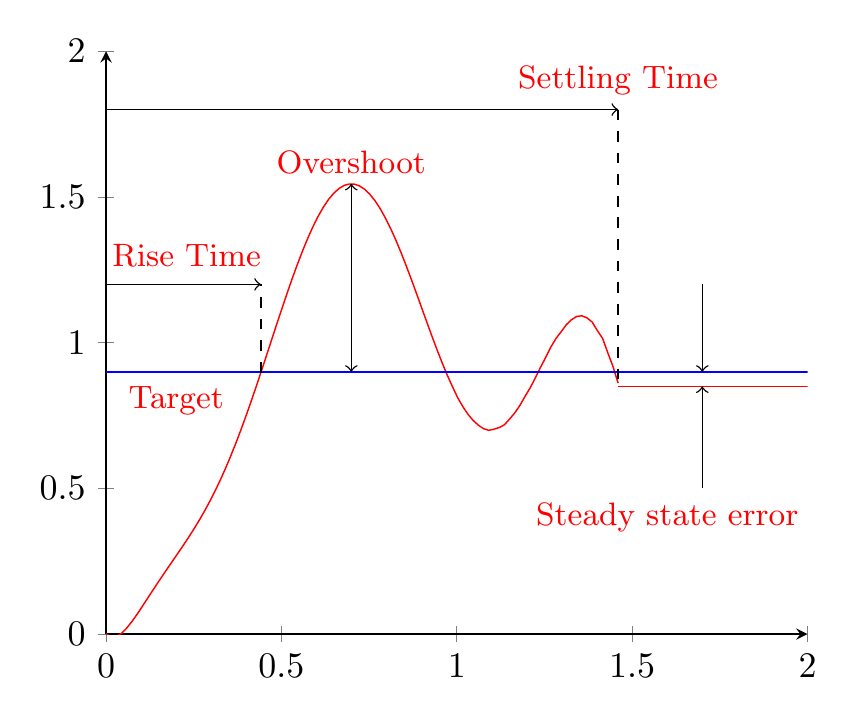
\begin{tikzpicture}[scale=1.3]
\begin{axis}[
    axis lines = left,
    xmin=0,xmax=2,
    ymin=0,ymax=2,
]

%Below the red parabola is defined
\addplot [
    domain=0:1.46, 
    samples=100, 
    color=red,
]
{80.83892322*x^8-473.66979127*x^7+1095.0629877*x^6-1265.55113227*x^5+768.48166718*x^4-242.51503181*x^3+39.47160828*x^2-1.30063244*x+0.00131008};

\addplot[color=red, domain=1.46:2] coordinates {
		(1.4598,0.85)
		(2,0.85)
};
\addplot[color=blue, domain=0:2] coordinates {
		(0,0.9)
		(2,0.9)
};
\addplot[<->,color=black, domain=0:2] coordinates {
		(0.69925398,1.5451)
		(0.69925398,0.9)
};

\node[red] at (axis cs:0.69925398,1.62){\small{Overshoot}};

\addplot[->,color=black, domain=0:2] coordinates {
        (1.7,1.2)
		(1.7,0.9)
};
\addplot[->,color=black, domain=0:2] coordinates {
        (1.7,0.5)
		(1.7,0.85)
};
\node[red] at (axis cs:1.6,0.4){\small{Steady state error}};

\addplot[color=black, domain=0:2, dashed] coordinates {
		(0.4415,0.8976)
		(0.4415,1.2)
};
\addplot[->,color=black, domain=0:2] coordinates {
		(0,1.2)
		(0.4415,1.2)
};
\node[red] at (axis cs:0.23,1.3){\small{Rise Time}};

\addplot[color=black, domain=0:2, dashed] coordinates {
		(1.4598,1.8)
		(1.4598,0.85)
};

\addplot[<-,color=black, domain=0:2] coordinates {
		(1.4598,1.8)
		(0,1.8)
};

\node[red] at (axis cs:0.2,0.8){\small{Target}};

\node[red] at (axis cs:1.4598,1.9){\small{Settling Time}};
\end{axis}
\end{tikzpicture}
\caption{PID properties.}\label{pidsettling}
\end{figure}